\documentclass[12pt]{article}
\usepackage[english]{babel}
\usepackage[utf8x]{inputenc}
\usepackage[T1]{fontenc}
\usepackage{scribe}
\usepackage{listings}
\usepackage{algorithm2e}
\Scribe{\small{Group 3, Group 4}}
\Lecturer{Abir De}
\RestyleAlgo{ruled}
\LectureNumber{2}
\LectureDate{August $8^{th},2022$}
\LectureTitle{Overview of Linear Algebra for ML}

\lstset{style=mystyle}

\begin{document}
	\MakeScribeTop

%#############################################################
%#############################################################
%#############################################################
%#############################################################

Linear Algebra is one of the key fundamental concepts required in Machine Learning. Uses of Linear Algebra include  modelling a system as a linear transformation of input data, helping solve a system of linear equations, data compression using Principal Component Analysis, etc. 
\section{Vectors and their Properties}
Vectors are the basic representation unit of a data-point , an ordered tuple of numbers. 
We start with few basic notations, properties, and functions that can be applied to vectors.
% Here's a citation~\cite{Kar84a}.

\subsection{Dot product}
\begin{definition}
The dot product of two equi-dimensional vectors $\textbf{u , v} \in \mathbb{R}^n$ is given by 
\begin{align*}
     \mathbf{u}\cdot \mathbf{v} &= \sum u_iv_i\\
    &= \mathbf{u^T} \mathbf{v}\\
\end{align*}
where $x_i$ denotes the $i^{th}$ component of vector $x$, and $x^T$ represent the transpose of a vector. In the above definition of dot product, it has been assumed that the vectors are represented as columns.  
\end{definition}
\subsection{Independence}
A set of vectors $\mathbf{v_1 , v_2} , \hdots , \mathbf{v_n}$ is said to be linearly independent if one cannot be represented by any linear combination of other vectors. 
More formally,
\begin{definition}
a set of vectors $\mathbf{v_1 , v_2} , \hdots , \mathbf{v_n}$ is said to be linearly independent iff for scalars $c_i$'s we have,
$$
    \sum_{i=1}^n c_i\mathbf{v_i} = 0 \implies c_i = 0 \qquad\forall i \in [1,n]
$$
\end{definition}
The above definition can also be seen that the solution of the equation $$
\mathbf{A}\mathbf{c} = \mathbf{0} $$
is only the trivial solution $c=0$, where is the matrix $\mathbf{A} = [\mathbf{v_1} ~\mathbf{v_2} ~ \hdots ~\mathbf{v_n}]$
\pagebreak
\subsection{Vector space}
A set of vectors \textbf{V} is said to qualify as a vector space if it is closed under the operations of addition and scalar multiplication i.e. :
\begin{definition}
A set of vectors $\mathbf{V}$, is said to be a vector space , if for any two vectors $\mathbf{u} , \mathbf{v} \in \mathbf{V}$ we have 
\begin{align}
   & a  *\mathbf{u} \in \mathbf{V} ,&a \in \mathbb{R}\\
    &a* \mathbf{u} + b*\mathbf{v} \in \mathbf{V} , &a,b \in \mathbb{R}
\end{align}
\end{definition}

\begin{definition}
If a subset $\mathcal{V_S}$ of any vector space $\mathcal{V}$ is itself a vector subspace then we say that it is a subspace of $\mathcal{V}$.
\end{definition}

An example of a vector space is $\mathbb{R}^n~  \forall n>0$.
\begin{figure}[h!]
\begin{center}
  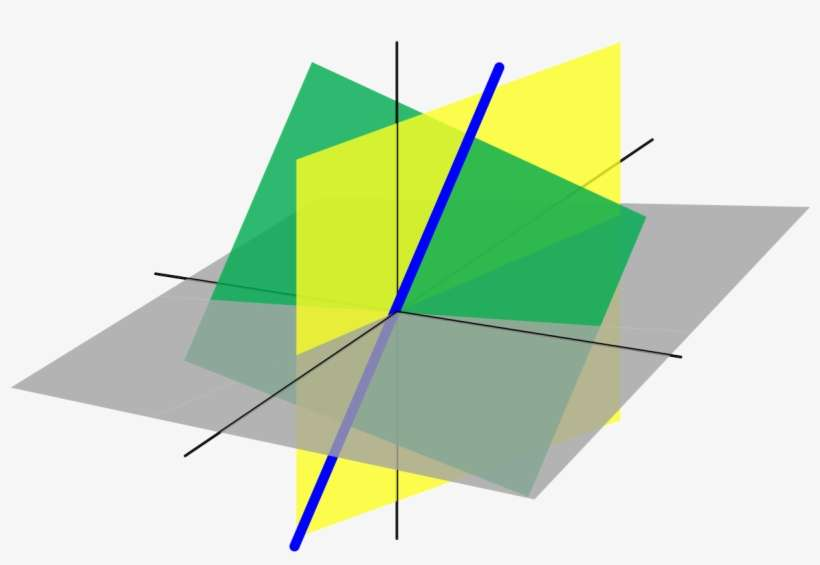
\includegraphics[width=0.4\linewidth]{LinSub.jpg}
  \caption{Examples of linear subspaces of $\mathbb{R}^3$}
\end{center}
\end{figure}
A subset of independent vectors of a vector space of highest cardinality is called a \textbf{basis} for the vector space. Every vector in the vector space can be represented as a linear combination of some or all vectors in a basis of the vector subspace. Note that the basis need not be unique for the vector space.

\section{Matrices}
A matrix is a rectangular array or a table of numbers, symbols , or expressions, arranged in rows and columns, which is used to represent a mathematical object or a property of such an object. Matrices form a fundamental part of linear algebra which have geometric meaning associated to them while dealing with data in Machine Learning. \\
An N $\times$ M matrix has N rows and M columns. Following is an example of a 2x2 matrix A.
$$ A = 
\begin{bmatrix}
1 & 2 \\
3 & 4 \\
\end{bmatrix}
$$

Any point in $\mathbb{R}^n$ can be seen as an $n$ dimensional vector, wherein multiplying a matrix with a vector then has the geometric significance of \textbf{applying a linear operation} on the vector.

\subsection{Matrix Multiplication}
\begin{definition}
If V is a matrix of size n $\times$ m and W is an m $m \times p$ matrix, then the matrix product U = VW is a size of $n \times p$ and can be computed as follows: 
$$V = \begin{bmatrix}
    v_{1,1} & \dots & v_{1,m} \\
    \vdots & \vdots & \vdots \\
    v_{n,1} & \dots & v_{n,m}
\end{bmatrix}
, 
W = \begin{bmatrix}
    w_{1,1} & \dots & w_{1,p} \\
    \vdots & \vdots & \vdots \\
    w_{m,1} & \dots & w_{m,p}
\end{bmatrix}
,
U = \begin{bmatrix}
    u_{1,1} & \dots & u_{1,p} \\
    \vdots & \vdots & \vdots \\
    u_{n,1} & \dots & u_{n,p}
\end{bmatrix}$$
\\
where $u_{i,j} = \sum_{k=1}^m v_{i,k}w_{k,j}$  
\end{definition}
\subsection{Determinants}
Determinant is a scalar value that is a function of the entries of a square matrix. In the case of a 2x2 matrix the determinant can be defined as 
$$
|A| \  = \ \begin{vmatrix}
a & b \\
c & d \\
\end{vmatrix}
\ =  \ ad - bc
$$
Higher order determinants recursively follow. 
\subsection{Linear Systems}
A linear system or a system of linear equation is a collection of one or more 
linear equations involving the same variables. A general system of linear equation with n unknows and coefficients can be written as \\
$$ a_{11}x_1 + a_{12}x_2 + \dots + a_{1n}x_n = b_1 $$
$$ a_{21}x_1 + a_{22}x_2 + \dots + a_{2n}x_n = b_2 \\ $$
$$\vdots $$
$$ a_{m1}x_1 + a_{m2}x_2 + \dots + a_{mn}x_n = b_m \\ $$
We can represent a system of linear equations using a coefficient matrix A, a vector of variables $\mathbf{x}$ and constants $\mathbf{b}$ as $: \mathbf{Ax = b}$. The problem then reduces to finding an x for a given A and b.


\section{Solving System of Equations}
A system of linear equations in n variables can have the following solutions :
\begin{itemize}
    \setlength\itemsep{0.0125em}
    \item Exactly one solution
    \item No solution
    \item An infinite number of solutions
\end{itemize}

\subsection{Matrix Inversion}
Given a linear system of equation represented by Ax = b, we can find a solution x = $A^{-1}b$, where $A^{-1}$ is called the inverse of the matrix.
\begin{itemize}
    \item If  $\mathbf{A}$ is invertible we can find unique solution to our systems of equation. 
    \item \textbf{Gauss-Jordan : } We perform elimination step on the augmented matrix [A I] to give the augmented matrix [I $A^{-1}$]. Gauss-Jordan elimination gives a Reduced Row Echelon Form.
    An \textbf{augmented matrix} $A|b$ is basically
    \begin{equation*}
    \begin{bmatrix}
    	a_{1, 1} & a_{1, 2} & \cdots & a_{1, n} & \vline & b_1\\
    	\vdots & \vdots & \vdots & \vdots & \vline & \vdots\\
    	a_{m, 1} & a_{m, 2} & \cdots & a_{m, n} & \vline & b_m \\
    \end{bmatrix}
    \end{equation*}
\end{itemize}



\subsection{Gaussian Elimination}
Given a system of linear equations denoted by
$$
\mathbf{A} x = \mathbf{b}
$$
we can solve the equations using Gauss Jordan Elimination. We note the elementary row operations are given as swapping two rows in the matrix , multiplying rows by a constant factor , and adding two rows. After performing Gaussian Elimination on the coefficient matrix we get a Row Echelon Form.

\begin{algorithm}
\caption{Gaussian Elimination}
\KwData{$\mathbf{A} , \mathbf{b}$}
\KwResult{$\mathbf{X}=[X_1 X_2 \dots X_n] \text{  such that  } \mathbf{A}\mathbf{X} = \mathbf{b}$}
$A\_b \gets A|b$\;
\tcc{Indexing assumed to start from 1}
$n \gets A.shape[1]$\;
\tcc{Forward Elimination }
\For{$i$ in 1 to n-1}{
  \tcc{Identify pivot}
  \eIf{$A\_b[i][i]$ is 0}{
    \tcc{Note: There is a variation of the algorithm where you move on to the next column if encountering zero}
    $X \gets$ "No solution exists"\;
  }{
  \For{$j$ in i+1 to n}{
  \For{$k$ in 1 to n+1}{
      $A\_b[j][k] \gets A\_b[j][k] - A\_b[j][i] / A\_b[i][i] * A\_b[i][k]$\;
      }
    }
 }
}
\tcc{Back Substitution }
$X_n \gets A\_b[n][n+1]/A\_b[n][n]$\;
\For{$i$ in n-1 to 1}{
$X_i \gets A\_b[i][n+1]$\; 
\For{$j$ in i+1 to n}{
$X_i \gets X_i - A\_b[i][j]*X_j$\;}
$X_i \gets X_i/ A\_b[i][i]$\;
}
\end{algorithm}

\subsection{LU decomposition and application}
We can also solve for the system of linear equations $Ax  = b$, by first converting $\mathbf{A}$ into a product of two matrices, such that one is completely a lower triangular matrix L and other is an upper triangular matrix U,
$$
A = LU$$
Matrix L and U , can be found by the help of Gaussian Elimination applied on the matrix A. Once we have L and U , we can then solve for x by first solving the equation , $$
L y = b$$
for y , and then the equation $$
Ux = y$$
\section{Column space, Null space and Invertibility}

\subsection{Column space :}\\ \\
Column space of a matrix $A$, or $C(A)$, is the space consisting of all possible linear combinations of the columns of $A$. For any real vector $x$, $Ax$ will lie in the column space of $A$.

\begin{itemize}
    \item If there exists a solution for the equation $b = Ax$ for a real matrix $A$ and real vectors $b$ and $x$,  then $b$ lies in the $C(A)$ and vice versa.
\end{itemize}
\\ \\
\subsection{Null space :}\\ \\
Null space of a matrix $A$, or $N(A)$, is the space spanned by all the solutions $x$, of $Ax = 0$.
\\ \\
The solutions form a vector space because :
\begin{itemize}
    \item $\text{If } Ax = 0 \text{ then } A(cx) = c(Ax) = 0$ 
    \item $\text{If } Ax = 0 \text{ and } Ay = 0 \text{ then } A(x + y) = 0$
\end{itemize}
\\
Having a vector $x$ other than the null vector, such that $Ax = 0$, implies that the columns of matrix $A$ are dependent.

\subsection{Rank of a matrix :} \\\\
Rank of a matrix $A$ is defined as the size of the maximal set of independent columns of the matrix $A$, and those columns form a basis for $C(A)$.

\begin{itemize}
    \item If $A^{-1}$ exists, the only solution to $Ax = b$ is $x = A^{-1}b$
    \item In addition to the first statement, $A$ is singular iff there are solutions other than $x = 0$ to $Ax = 0$, or in other words, iff it has a non-singular null-space $N(A)$.
\end{itemize}
\\A matrix $A$ is called a full column rank matrix if all the columns in $A$ are independent.

\subsection{Invertibility :}\\
A square matrix $A$ is invertible if there exists a square matrix $B$ such that $AB = BA = I_{n}$, and $B$ is known as inverse of $A$, also denoted by $A^{-1}$.
\begin{itemize}
    \item A square matrix is invertible iff it is a full column rank matrix.
\end{itemize}

\subsection{Computing the Inverse - Gauss Jordan Elimination :}

The Gauss-Jordan elimination method addresses the problem of solving several linear systems $Ax_{i} = b_{i}  (1 \leq i \leq N)$ at once, such that each linear system has the same coefficient matrix $A$ but a different right hand side $b_{i}$.
\\\\
We have seen how elimination matrices are used to convert a coefficient matrix $A$ into some upper triangular matrix $U$,

$$U = E_{32}(E_{31}(E_{21}A)) = (E_{32}E_{31}E_{21})A$$
\\
Now, further apply elimination steps until $U$ gets transformed into identity matrix:

$$I = E_{13}(E_{12}(E_{23}(E_{32}(E_{31}(E_{21}A))))) = (E_{13}E_{12}E_{23}E_{32}E_{31}E_{21})A$$
\\
By definition, $X = (E_{13}E_{12}E_{23}E_{32}E_{31}E_{21})$ must be $A^{-1}$
\\ \\
Note that the above method works only if $A$ is invertible.
\\ \\
So, Gauss-Jordan is basically elimination steps over the augmented matrix $[A I]$ (representing the equation $AX = I$) to give the augmented matrix $[I A^{-1}]$ (representing the equation $IX = A^{-1}$)

\subsection{Dealing with Rectangular matrices :}
What if $A$ is not a square matrix but rather a rectangular matrix of size $m x n$, such that $m \neq n$. Does there exist a notion of $A^{-1}$? The answer depends on the rank of A.
\begin{itemize}
    \item If $A$ is full row rank and $n > m$, then $AA^{T}$ is a full rank $m x m$ matrix $\Longleftrightarrow (AA^{T})^{-1}$ exists with $A^{T}(AA^{T}^{-1})$ leading to $I$ and is therefore called the right inverse of A. When the right inverse of $A$ is multiplied on its left, we get the projection matrix $A^{T}(AA^{T})^{-1}A$, which projects matrices onto the row space of $A$.
    \item If $A$ is full column rank and $m > n$, then $A^{T}A$ is full rank $n x n$ matrix $\Longleftrightarrow (A^{T}A)^{-1}$ exists with $(A^{T}A)^{-1}A^{T}$ leading to $I$ and is therefore called the left inverse of A. When the left inverse of $A$ is multiplied on its right, we get the projection matrix $A(A^{T}A)^{-1}A^{T}$, which projects matrices onto the column space of $A$.
\end{itemize}
\\
If $A$ is a full column rank matrix (that is, its columns are independent), $A^{T}A$ is invertible.
\\\\
We will show that the null space of $A^{T}A$ is ${0}$, which implies that the square matrix $A^{T}A$ is full column (as as well as row) rank is invertible. That is if $A^{T}Ax = 0$, then $x = 0$. Note that if $A^{T}Ax = 0$, then $x^{T}A^{T}Ax = ||Ax|| = 0$ which implies that $Ax = 0$. Since the columns of A are linearly independent, its null space is 0 and therefore, $x = 0$.
%%%%%%%%%%% If you don't have citations then comment the lines below:
%
% \bibliographystyle{abbrv}           % if you need a bibliography
% \bibliography{mybib}                % assuming yours is named mybib.bib


%%%%%%%%%%% end of doc
\end{document}